% due July 8
\DocumentMetadata{
  lang=en,
  tagging=on,
  pdfstandard=ua-2,
%  check-tagging-status,
  tagging-setup={
%    math/alt/use,
    math/setup=mathml-SE
  }
}
\documentclass{ltx-talk}

\date{July 2026}
\title[Accessible PDF Textbook]{Converting a PDF Textbook to be Accessible}
\author[Tim Prescott]{Timothy Prescott (\TeX.SE: \texttt{teepeemm})}
\subtitle{Anyone can do it}
\institute{University of North Dakota}
% abstract:
%A guideline in the United States requires that
%\acro{PDF}s created after April 2026 must be accessible to visually
%impaired users. We discuss how we updated a custom three semester
%calculus book to be accessible, including what we did, the challenges we
%faced, how we verified accessibility, and what remains to be done. We
%also discuss necessary adaptations to satisfy a common accessibility
%checker available in several \acro{LMS}s.

% 30 minutes including questions

\usepackage{booktabs}
\usepackage{siunitx}
\usepackage{emoji}
\usepackage{tikz-cd}
\usepackage{pgfplots}
\usepackage{listings}

\DeclareMathOperator{\coker}{coker}
\pgfplotsset{compat=1.18}

\newcommand{\apex}{\texorpdfstring{A\kern -.1em \lower -.5ex\hbox{P}\kern -.25em\lower .5ex\hbox{E}\kern -.1em X}{APEX}}

\ProvideDocumentEnvironment{tcb@manual@entry}{}{}{} % needed for the next line
\usepackage{tagpdfdocu-patches}% needed to make listings work properly

\lstset{
  columns=fullflexible,
  keepspaces=true,
  commentstyle=\slshape,
  basicstyle=\ttfamily
  \lst@ifdisplaystyle\small\fi,
  language={[LaTeX]TeX}
}

\newcommand{\cs}[1]{\texttt{\textbackslash #1}}
\newcommand{\tubbraced}[1]{\texttt{\{#1\}}}
\newcommand{\meta}[1]{\ensuremath{\langle}%
 \ifmmode\expandafter\mbox\fi{\itshape #1\/}%
 \ensuremath{\rangle}%
}

%\providecolor{maybeUNDgreen}{Hsb}{146,1,0.62}
\providecolor{maybeUNDgreen}{Hsb}{146,1,0.53}

\EditInstance{header}{std}{
    background-color = maybeUNDgreen,
    color            = white,
}

\DeclareInstance{footer-element}{frameoftotal}{talk}{}
\ExpandArgs{c}\newcommand{@frameoftotal}{%
  \arabic{frame}/\RefProperty{lastpage}{totalframes}
}
\EditInstance{footer}{std}{
  color         = black!75,
  separator     = \hfill|\hfill,
  element-order = {date, author, title, frameoftotal},
}

\DeclareInstance{titlepage-element}{titlegraphic}{talk}{}
% department logo obtained locally
% other graphics from https://campus.und.edu/brand/downloads.html
% primary logotype, full color, svg converted to pdf
\ExpandArgs{c}\newcommand{@titlegraphic}{%
  \addvspace{\medskipamount}
  
\includegraphics[
    actualtext={University of North Dakota, Mathematics \& Statistics},
    width=5cm
  ]{MathStats-CMYK_primary.jpg}% logotype-full
  \addvspace{\smallskipamount}
}
% flame logo, white, digital png
\newsavebox\logobox
%\savebox\logobox{\includegraphics[artifact, height=2ex]{example-image}}
\savebox\logobox{%
  
\includegraphics[artifact, height=\baselineskip]{flame-w-rgb}}
\AddToHook{shipout/foreground}{%
  \put(\paperwidth - \wd\logobox - 10mm,
       -8.5mm){\usebox\logobox}} % -\ht\logobox
%\NewCommandCopy\oldframetitle\frametitle
%\RenewDocumentCommand{\frametitle}{m}{%
%  \oldframetitle{#1\hfill
%    
\includegraphics[height=2ex,artifact]{flame-w-rgb}%
%  }%
%}

\begin{document}

\begin{frame}
\maketitle[
  element-order = {title, author, titlegraphic, date},
  framestyle = plain
]
\end{frame}

\begin{frame}
\frametitle{A Strangely Sporadic Timeline}
\newlength{\maxwidth}
\setlength{\maxwidth}{\widthof{2024-04-26\ \ }}
\begin{description}[
  label-width=\maxwidth,
  label-align=left,
%  left-margin=10em,
  left-margin=\maxwidth,
]
\item[1978] \TeX
\item[1990] Americans with Disabilities Act (ADA). \\
Title II: Government entities may not discriminate\\
against those with disabilities.
\item[1993] PDF
\item[2016] University of North Dakota adopts \apex\ Calculus.
\item[2017--2020] PDF 2.0 (better math support).
\item[2019] \LaTeX\ team begins improving accessibility in earnest
\item[2024-04-26] US Dept of Justice: ADA Title II means that\\
public entities must make documents accessible.\\
Most entities get two years.  We (DoJ) get three years.
\item[2026-04-20] Everyone gets an extra year.
\end{description}
\end{frame}

\begin{frame}
\frametitle{Basic Outline of Accessibilizing}
\tableofcontents
\end{frame}

\begin{frame}
\frametitle{Basic Table of Accessibilizing}
\sisetup{table-format=3}
\tagpdfsetup{table/header-rows={1,2}}
\begin{tabular}{@{} l @{\qquad} SSS @{\qquad} S @{}}
Topic & \multicolumn{3}{c}{Time spent (\%)\quad\ } & {How accessible} \\
& {on the textbook} & {today} & {on your own} & {(\%)} \\\midrule
Preamble & 3 & 10 & <1 & 85 \\
Images & 20 & 30 & 25 & 5 \\
Tables & 17 & 30 & 25 & 5 \\
All else & 60 & 30 & 50 & 5 \\\midrule
 & 100 & 100 & 100 & 100
\end{tabular}
\end{frame}

\section{Preamble}

\begin{frame*}
\frametitle{TL;DR}
Update \LaTeX
\begin{lstlisting}
\DocumentMetadata{
  lang=en,
  tagging=on,
  pdfstandard=ua-2,
% check-tagging-status,
  tagging-setup={
%    math/alt/use,
    math/setup=mathml-SE
  }
}
\documentclass{...}
\usepackage{unicode-math}
\end{lstlisting}
compile with Lua\LaTeX, and most of the work is done\\
\texttt{texdoc documentmetadata-support-code}
\end{frame*}

%\section{How to \TeX\ an accessible PDF}

\begin{frame*}
\frametitle{Basic idea}
Use good \LaTeX\ so that the output looks how you want it\\
\emph{and the input reflects the meaning.}
\begin{itemize}
\item Aim for a clean log
\item Don't use tabular to position boxes.
\end{itemize}
Make use of \emph{semantic} macros and environments:\\
Bad: \verb|\textbf{Example 3.1.4 Finding Extreme Values}|\\
Good: \verb|\begin{example}{Finding Extreme Values}|\\
% \end{example}
Prefer environments over macros
\end{frame*}

\section{Images}

\begin{frame}
\frametitle{What Else to do --- Images}
\begin{itemize}
\ttfamily
\item\cs{includegraphics}[\textbf{alt=\tubbraced{...}}]
\item\cs{tikz}[\textbf{alt=\tubbraced{...}}]
\item\cs{begin}\tubbraced{tikzpicture}[\textbf{alt=\tubbraced{...}}]
\item\cs{begin}\tubbraced{picture}[\textbf{alt=\tubbraced{...}}]
\end{itemize}
Keep it brief and objective; exposition won't be seen by most readers\\
Alternatives to {\bfseries\ttfamily alt=\tubbraced{...}} are
\begin{itemize}
\item {\bfseries\ttfamily artifact} (image is decorative only)\quad
\colorbox{maybeUNDgreen}{
\includegraphics[height=2ex,artifact]{flame-w-rgb}}
\item {\bfseries\ttfamily actualtext=\tubbraced{...}}
(image is text in disguise)
\quad
\raisebox{-.8\height}{%
  
\includegraphics[
    actualtext={University of North Dakota, Mathematics \& Statistics},
    width=5cm
  ]{MathStats-CMYK_primary.jpg}% logotype-full
}
\end{itemize}
%\\
%PAC objects to a bug in pgfplots.
\end{frame}

\begin{frame*}
\frametitle{Alt Text}
\begin{itemize}
\item Usually not seen
\item Specific, accurate, objective, neutral
\item What does my audience need from this picture?
\item How would I tell someone to draw this picture?
\item Do not begin with ``image''
\item Do not repeat the caption
\item At most 120 characters or 1--2 sentences.\\
If not possible, have the alt text point to a separately written description
\smallskip
%\item Backup method: \verb|\setkeys{Gin}{alt={...}}|
\item ``Formulas need alt text'' $\leftrightarrow$ option
\texttt{math/alt/use}
\item Have someone else write the alt text?
\end{itemize}
\end{frame*}

\begin{frame}
\frametitle{Alt Text Problem 1}
``What alt text would you give for the snake lemma?''\bigskip
\AddToHookNext{env/tikzcd/begin}{\MathCollectFalse}
\begin{tikzcd}[
    ampersand replacement = \&,
    alt={A complicated commutative diagram.},
    every label/.append style = {font = \small}
%    font=\footnotesize,
%    row sep=small,
%    column sep=tiny,
%    cramped,
  ]
  \& \& \ker(a) \ar{r} \ar{d}
  \& \ker(b)\ar{r} \ar{d}
  \& \ker(c) \ar{d}   %\arrow[ddll,"\delta",rounded corners
  \& \&\\
  \& \& A \ar{r}{f} \ar{dd}[near end]{a}
  \& B \ar{r}{g} \ar{dd}[near end]{b}
  \& C \ar{r}\ar{dd}[near end]{c} \& 0 \& ~\\
  \& \& \& ~ \& \& \ar[r, phantom, ""{coordinate, name=Y}] \&~\\
  ~\& \ar[l, phantom, ""{coordinate, name=Z}] 0 \ar{r}
  \& A' \ar{r}{f'} \ar{d}
  \& B' \ar{r}{g'} \ar{d}
  \& C' \ar{d} \& \& \\
  \& \&
  \ar[from=uuuurr, "d", crossing over, rounded corners,
      to path={ -- ([xshift=2ex]\tikztostart.east)
                -| (Y) [near end]\tikztonodes
                -| (Z) [near end]\tikztonodes
                |- ([xshift=-2ex]\tikztotarget.west)
                -- (\tikztotarget)}
     ]\coker(a)\ar{r}
  \& \coker(b) \ar{r}
  \& \coker(c) \& \&
\end{tikzcd}
\end{frame}

\begin{frame}
\frametitle{Alt Text Problem 1b}
\begin{minipage}{\textheight}
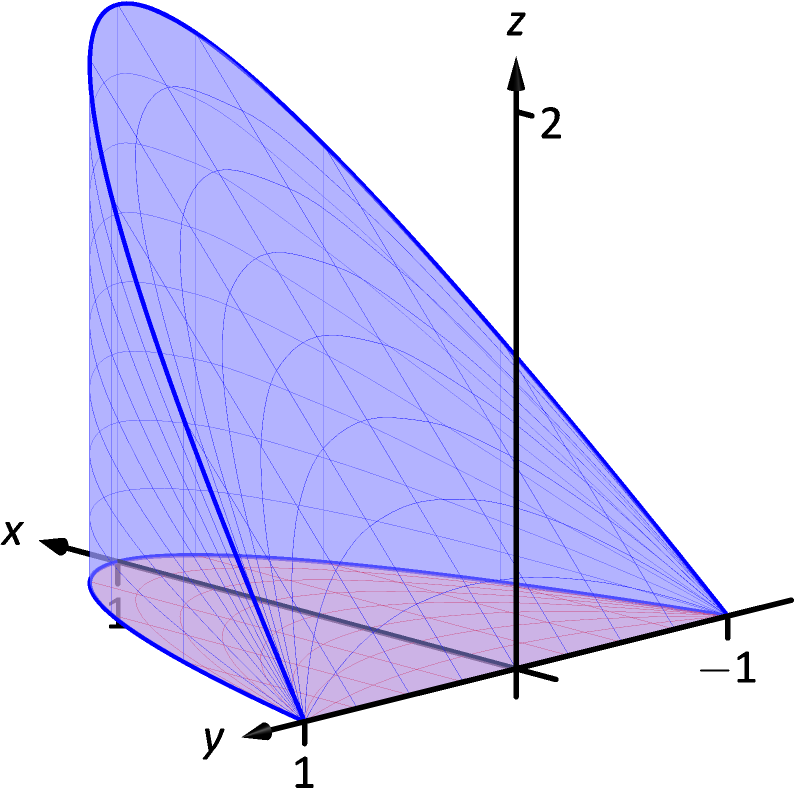
\includegraphics[width=\textheight,alt={An interactive 3d shape from the textbook.}]{figdivthm_space2_3D}
\end{minipage}\quad
\begin{minipage}{.4\textwidth}
Textbook feature:\smallskip\\
Asymptote + media9 \\
\null\quad\textrightarrow\ interactive 3d graphics
\end{minipage}
\end{frame}

\begin{frame}
\frametitle{Alt Text Problem 2}
  Exercise: Describe this function, identifying limiting values, intercepts
  and their degree, critical and inflection points,
  and regions where the function is increasing, decreasing, and
  concave up or down.

  \begin{tikzpicture}
  \begin{axis}[xmin=-2,xmax=2,ymin=-.1,ymax=1.6,width=\linewidth,
  axis x line=center,axis y line=center,axis equal image]
    \draw(-2,0.5)--(-1,1)circle(.04);
    \draw[fill=black](-1,0)circle(.04);
    \addplot[domain=-1:2,smooth]{.5*(x+1)*(x-1)^2};
  \end{axis}
  \end{tikzpicture}
\end{frame}

\section{Tables}

\begin{frame}
\frametitle{What Else to do --- Tables}
\begin{itemize}
\item\texttt{\cs{tagpdfsetup}\tubbraced{table/header-rows=\tubbraced{...},table/header-columns=\tubbraced{...}}\\
\qquad\qquad \textrm{outside of the} tabular\\
\qquad\qquad \textrm{(lasts until the group} \cs{ends})}
\item\texttt{\cs{tagpdfsetup}\tubbraced{table/multirow=\tubbraced{\meta{number of rows}}}} 
\item Interface will probably change
\item \texttt{texdoc latex-lab-table}
%\item Need to work around a PAC bug
%\item And PAC still doesn't like multi(row/column) in the data
\end{itemize}
\end{frame}

\section{All else}

\begin{frame}
\frametitle{Replacements \& Adjustments}
\begin{itemize}
\item enumitem \& enumerate \textrightarrow\ enumext or templates (\texttt{texdoc blocks-doc})
\item margin[fit|fix|note] \textrightarrow\ margin[alia|par]
\item titlesec \textrightarrow
\begin{itemize}
\item \cs{@startsection} (\texttt{texdoc latex2e}, \S6.8)
\item templates (\texttt{texdoc latex-lab-sec-template})
\end{itemize}
\item Beamer \textrightarrow\ ltx-talk (tomorrow)
\item Some packages need some (or a lot of) help (tcolorbox, qrcode, media9, \ldots)\\
use option \texttt{check-tagging-status} or\\
\url{https://latex3.github.io/tagging-project/tagging-status/}
\end{itemize}
\end{frame}

%\section{Testing}

\begin{frame}
\frametitle{Tools}
To verify that a PDF is accessible:
\begin{description}
%\item[Ally, Siteimprove:] (Commercial addons)
%\begin{itemize}
%\item[\emoji{thumbsup}] easy to pass, checks color contrast
%\item[\emoji{thumbsdown}] too easy, false negatives
%\end{itemize}
\item[Screen reader:] (NVDA or JAWS) and (Adobe, FoxIt, or Firefox)
\item[veraPDF:] \url{https://verapdf.org/software}
\begin{itemize}
\item[\emoji{thumbsup}] has command line version; \LaTeX\ team
\item[\emoji{thumbsdown}] no GUI for PDF errors
\end{itemize}
\item[PDFix:] \url{https://pdfix.net}
\begin{itemize}
\item[\emoji{thumbsup}] GUI
\item[\emoji{thumbsdown}] no command line
\end{itemize}
%\item[PAC:] \url{https://pac.pdf-accessibility.org/en}
%\begin{itemize}
%\item[\emoji{thumbsdown}] Windows only; maxes out at UA-1/1.7; bug with tabular headers
%\item[\emoji{thumbsup}\emoji{thumbsdown}] more thorough (pgfplots, multi[row|column])
%\end{itemize}
\end{description}
\end{frame}

% cut for MAA
%\section{Tools}

\begin{frame}
\frametitle{veraPDF --- \url{https://verapdf.org/software}}
%\centering
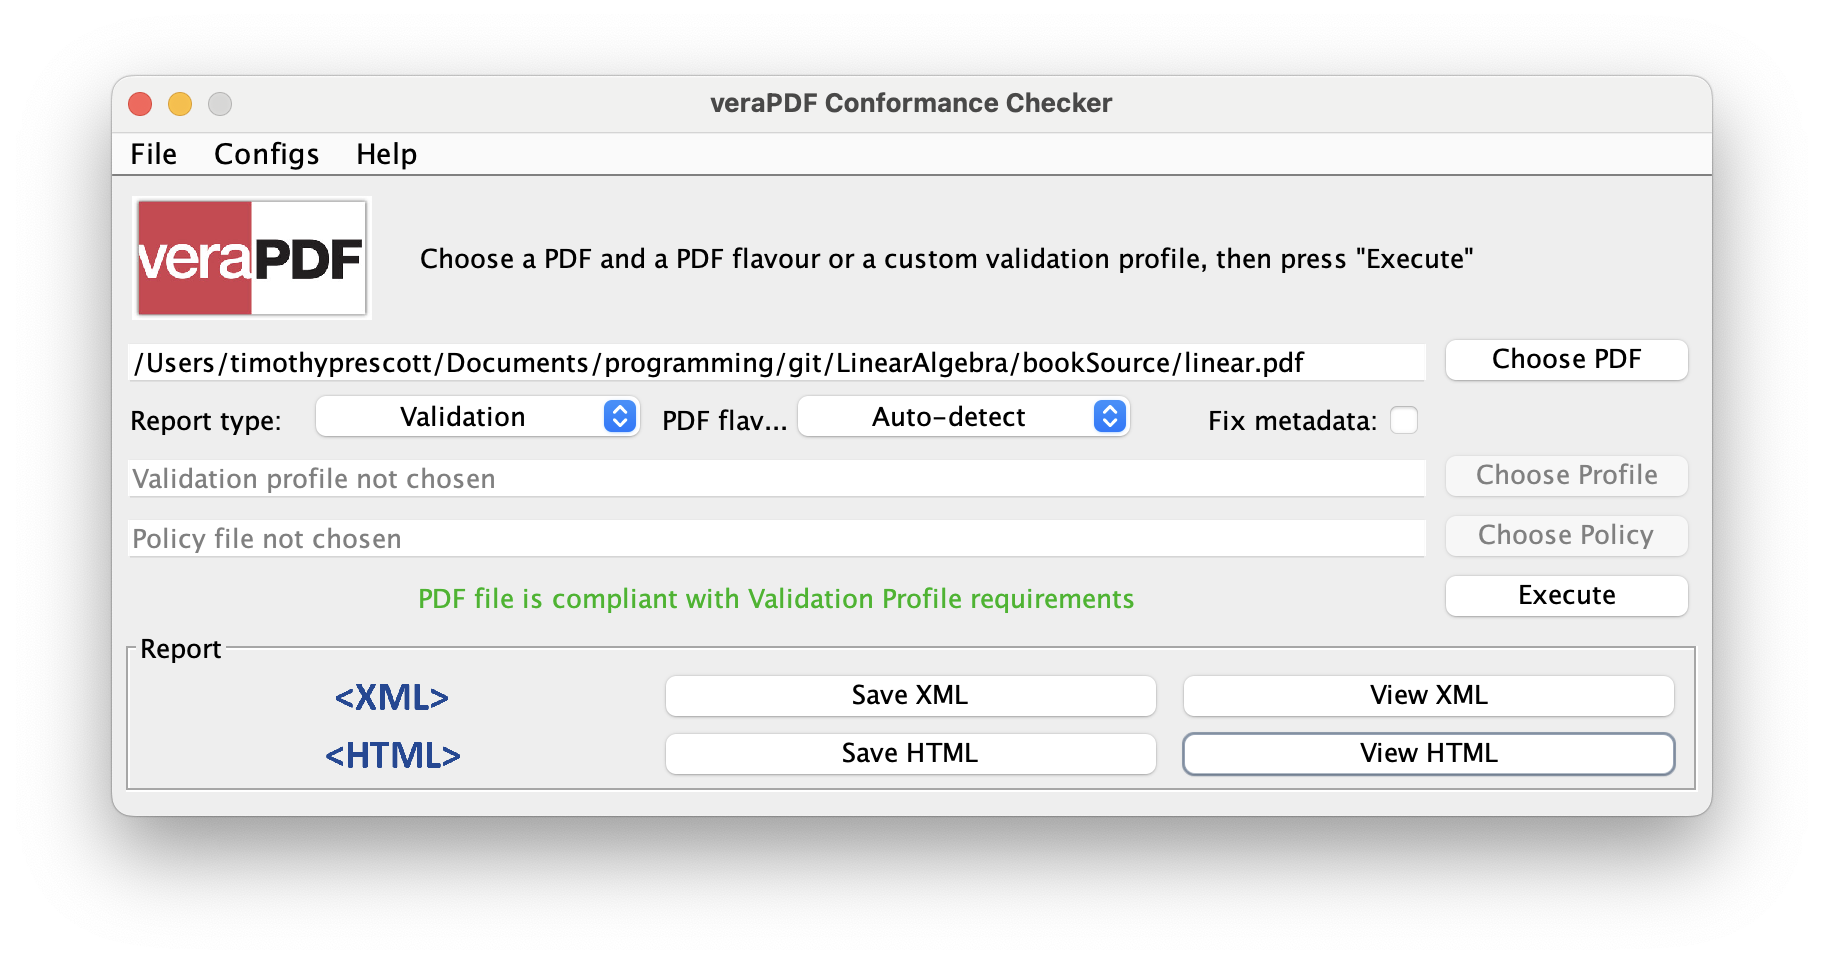
\includegraphics[alt={Screenshot of veraPDF},height=\textheight]{veraPdfScreenshot}
\end{frame}

\begin{frame*}
\frametitle{veraPDF --- Example Error}
\begin{verbatim}
root/
  document[0]/
  StructTreeRoot[0](5 0 obj PDStructTreeRoot)/
  K[0](22 0 obj SEDocument Document)/
  K[2130](24072 0 obj SESect figures)/
  K[71](102535 0 obj SEAside float)
\end{verbatim}
\end{frame*}

\begin{frame}
\frametitle{PDFix --- \url{https://pdfix.net}}
%\centering
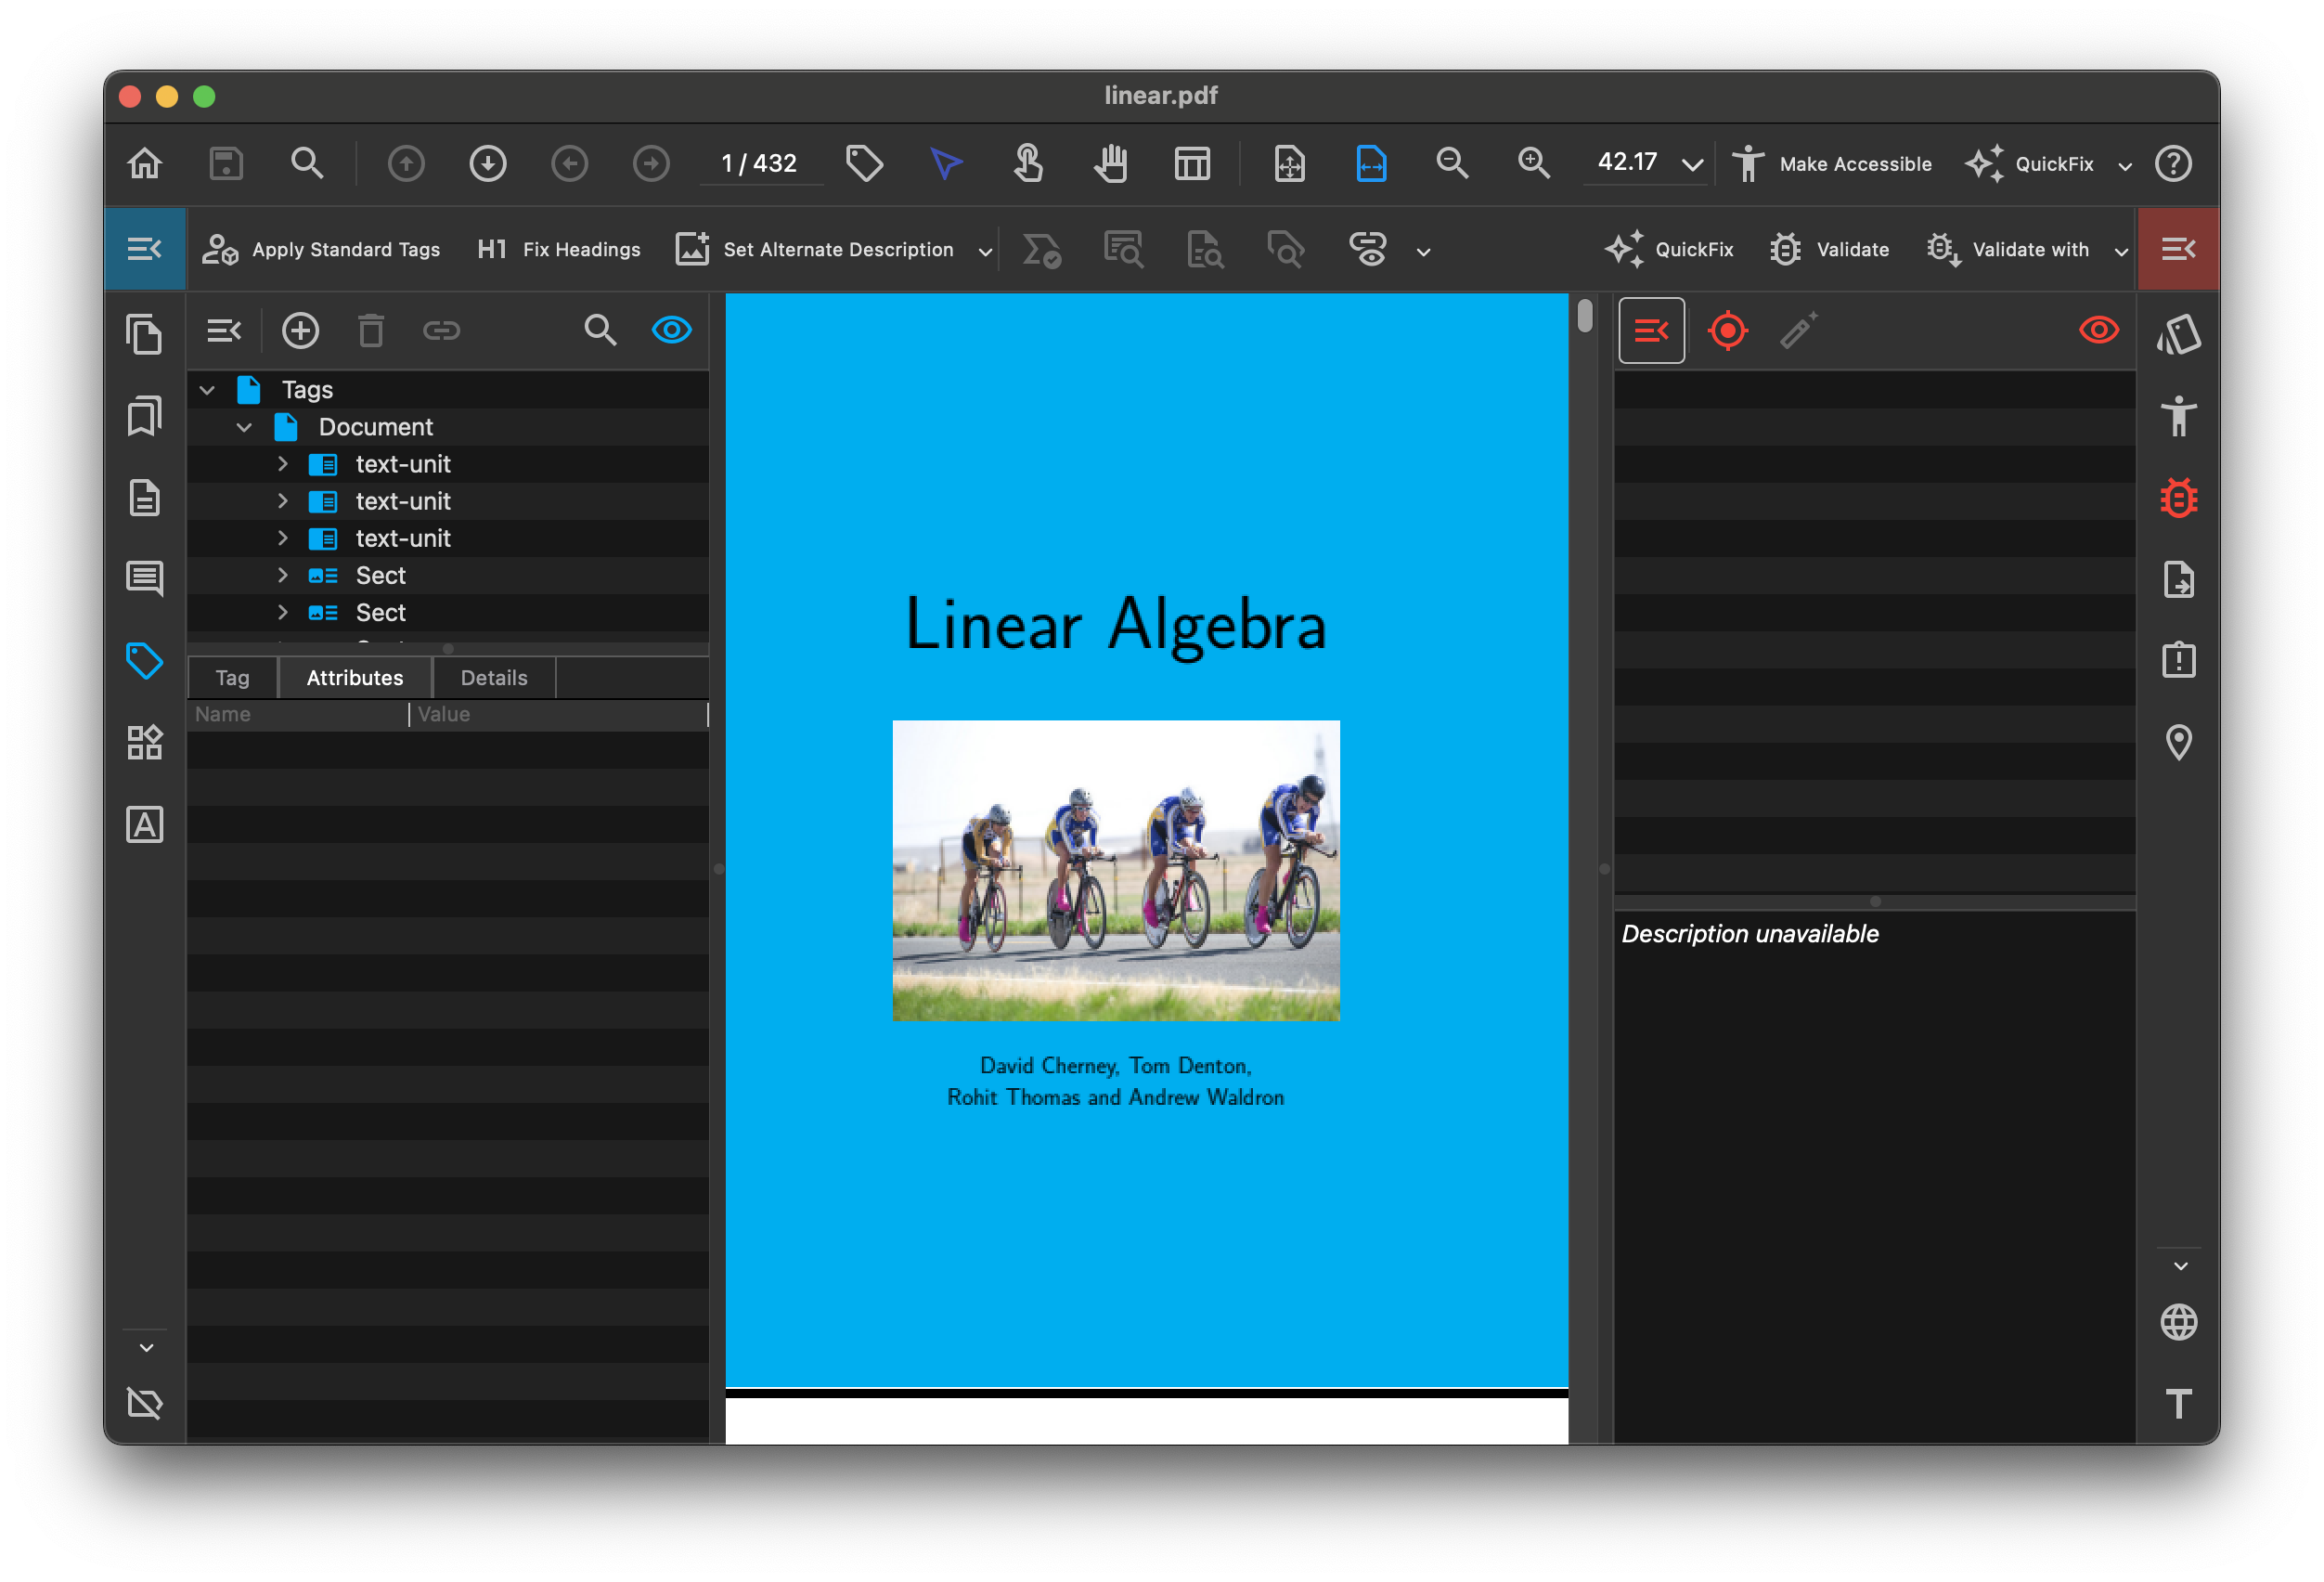
\includegraphics[alt={Screenshot of PDFix},height=\textheight]{pdfixScreenshot}
\end{frame}

\begin{frame}
\frametitle{PDFix --- Same Example Error}
%\centering
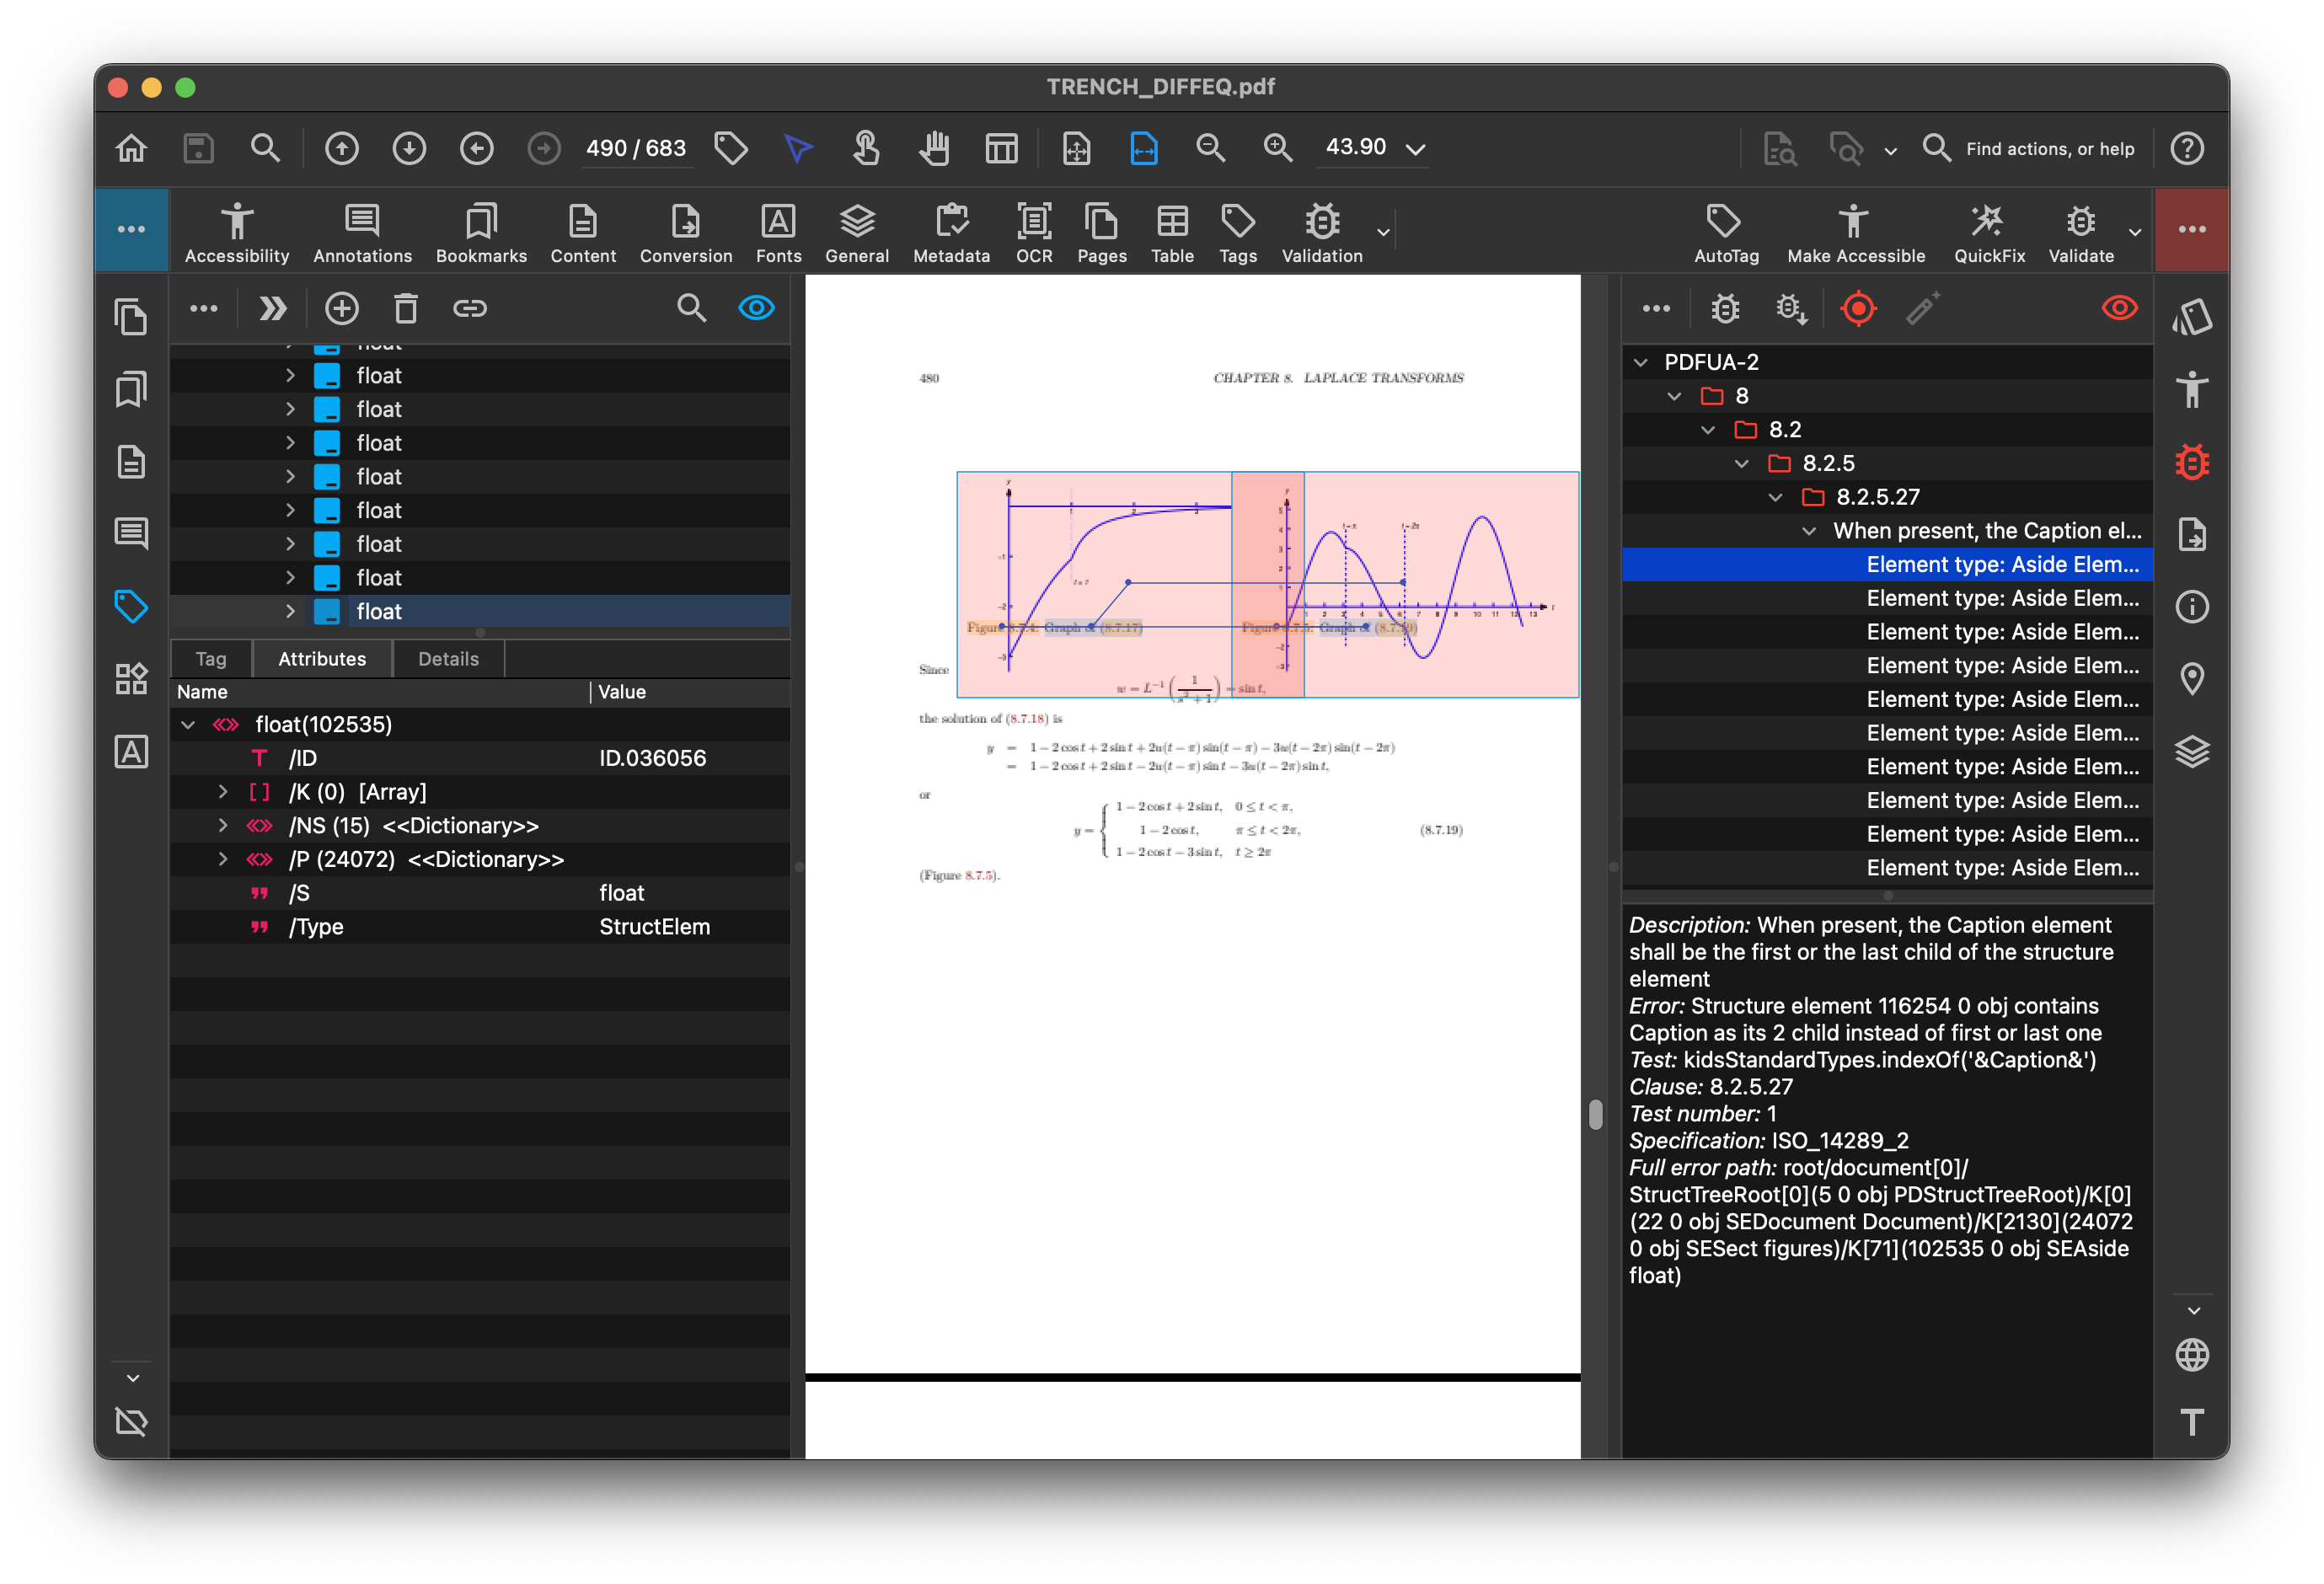
\includegraphics[alt={Screenshot of PDFix error},height=\textheight]{pdfixValError}
\end{frame}

%\begin{frame}
%\frametitle{PAC --- \url{https://pac.pdf-accessibility.org/en}}
%\centering
%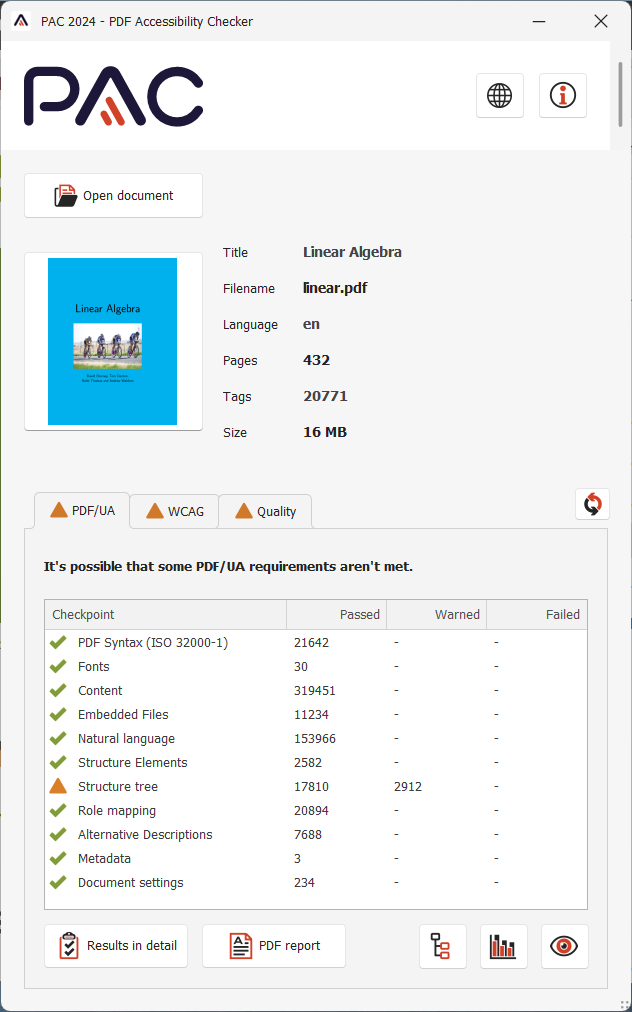
\includegraphics[alt={Screenshot of PAC},height=\textheight]{PacScreenshot}
%\qquad
%\raisebox{.5\textheight}{\parbox{.5\linewidth}{A bit more streamlined, but:
%\begin{itemize}
%\item Windows only
%\item maxes out at UA-1/1.7
%\item objects to bug in pgfplots
%\item has a bug with tables
%\item doesn't like multi(row/column)
%\end{itemize}
%\end{frame}

%\begin{frame*}
%\frametitle{ltx-talk}\pause
%\begin{itemize}[<+->]
%\item Same \verb|\pause|/overlay specification idea (eg, \verb|\begin{itemize}[<+->]|)
%\item ``\emph{highly} experimental'' --- must use \texttt{lualatex-dev} (for another month?)
%\item Ally $\Rightarrow$ \verb|\AtBeginDocument{\tagpdfsetup{role/new-tag=frametitle/H1}}|
%\item Can ``easily'' specify header and footer information\\\bigskip
%\hfill%
%\alt<+->{%
% 
\includegraphics[height=.4\textheight,alt={MALL presentation with logo in corner}]{Blackboard-PPT-Tues.pdf}%
%}{%
% \parbox[c][.4\textheight]{1em}{}%
%}%
%\hfill\null
%\end{itemize}
%\end{frame*}

%\section{For more information}

\begin{frame}
\frametitle{Misconceptions}
Email from IT:
\begin{quote}
``To keep it in the format (PDF) that it is in now would result in major \alert<3>{clean-up} to the tagging structure (\alert<3>{in Adobe} particularly). You could do it, but 1000 pages \alert<3>{in Adobe} is a lot \alert<3>{to remediate}. Additionally, the code in the content tab of Adobe has a lot of \alert<2>{rogue elements} that came over. There are \alert<2>{containers in there that don't even correspond to textual or visual elements on the page}, so I don't know where those came from; they must have resulted from something in the conversion process from LaTex to PDF.''
\end{quote}\bigskip
\begin{itemize}
\item<alert@2> Adobe checks PDF1.7, not PDF2.0
\item<alert@3> Remediation can be done at creation by \LaTeX, not after in Adobe
\item \texttt{.tex \textrightarrow\ .pdf} is not a one time process
\end{itemize}
\end{frame}

\begin{frame*}
\frametitle{Last Bits}
\begin{itemize}
\item \url{https://latex3.github.io/tagging-project/documentation/prototype-usage-instructions.html}
\item \url{https://github.com/teepeemm/accessibility}
\item Compiling needs more:\smallskip\\
\begin{tabular}{lS[table-format=2(1),uncertainty-mode=separate]}\toprule
Statistic & Factor \\\midrule
Time & 10(3) \\
RAM & 6(2) \\
Output size & 2(1) \\
strings & 11(4)\\
hash & 10(4)\\\bottomrule
\end{tabular}
\smallskip\\
Try \verb|\DocumentMetadata{tagging=off}| for draft runs
%\item \url{https://www.youtube.com/watch?v=Eu_qM53tInw&t=5900s}\\
%\qquad A before and after example using Foxit, NVDA, and MathCAT
\item Don't be afraid to edit beyond the preamble
\end{itemize}
\end{frame*}

\end{document}

\begin{frame}
\frametitle{Examples}\tagpdfsetup{table/header-rows={1}}
\begin{tabular}{l p{.2\textwidth} p{.5\textwidth}}
Math & before & after \\\midrule
$a^2+b^2=c^2$ & ay two plus bee two equals cee two & ay squared plus bee squared is equal to cee squared\\\addlinespace[4ex]
{$\begin{pmatrix}a&b\\c&d\end{pmatrix}^{-1}$} & minus one list with one item ay bee cee dee & two lines line one ay bee line two cee dee to the negative one power \\\addlinespace[4ex]
{$\begin{pmatrix}1&2\\3&4\end{pmatrix}\begin{pmatrix}1&1\\0&1\end{pmatrix}$} & three four one two zero one one one & the two by two matrix row one one two row two three four times the two by two matrix row one one one row two zero one
\end{tabular}
\end{frame}

% cut for MAA
%\begin{frame}
%\frametitle{Colors}
%\begin{itemize}
%\item UND green is $\operatorname{RGB}(0,158,68)=\operatorname{Hsb}(146,1,0.62)$
%\item UND orange is $\operatorname{RGB}(255,103,31)=\operatorname{Hsb}(19,0.88,1)$
%\item Insufficient contrast with white?
%\item Add 13\% and 22\% black.
%\item Also red with white (hyperref)
%\end{itemize}
%\end{frame}

\end{document}
